\documentclass{article}
\usepackage[utf8]{inputenc}
\usepackage{amssymb}
\usepackage{graphicx}


\title{IFT3335-TP1-Rapport}
\author{Wenhao Xu, 20150702\\
Mingze Li, \\
Yu Deng, 20151659}

\date{}

\begin{document}

\maketitle

\section*{Tâche 1 et Tâche 2}\\

On test \textbf{sudoku original.py}, qui est le fichier sudoku.py de Norvig, et on a le résultat suivants (prenez simplement une valeur, chaque résultat de test doit être différent) :\\
$#solve_all(from file("100sudoku.txt"), "95sudoku", None)$\\
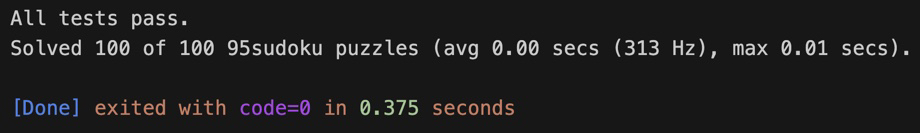
\includegraphics[scale=0.3]{t1_1.jpeg}\\
Avec "Choisir les carrés non remplis", On test \textbf{sudoku task2.py}, ceci revient à une recherche pure en profondeur d’abord sans aucune heuristique. Voici les résultats:\\
$#solve_all(from file("100sudoku.txt"), "95sudoku", None)$\\
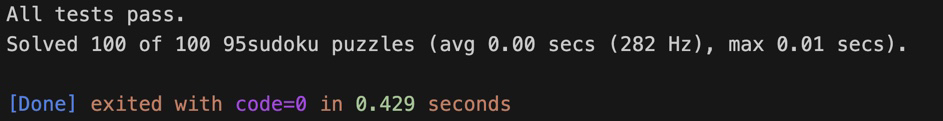
\includegraphics[scale=0.3]{t2_1.jpeg}\\

$\bullet$ Nous pouvons en déduire que pour le deuxième code, nous avons besoin d'un peu plus de temps, même si la différence n'est pas très grande, mais cela montre aussi l'importance de l'heuristique.

\section*{Tâche 3}\\
\\
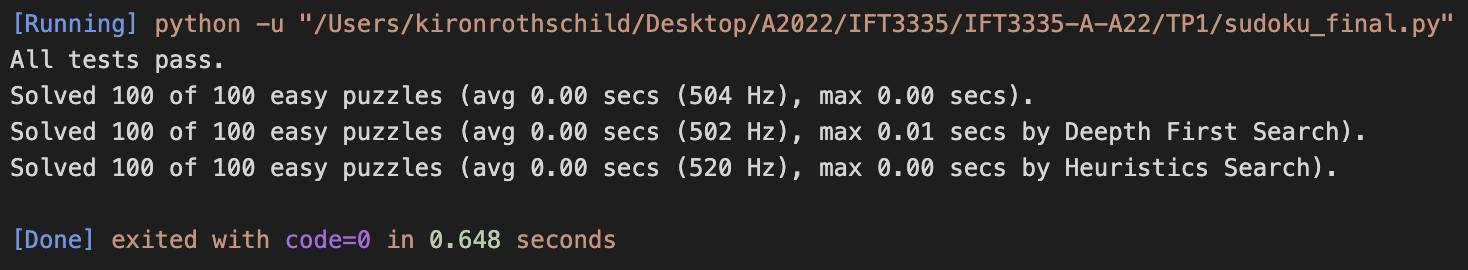
\includegraphics[scale=0.4]{t3.png}







\end{document}
